\chapter{相关工作}
本章将对本文的研究框架中所涉及的相关技术进行分析,主要分为三个方面:一个方面是介绍结构图表征的相关算法,也就是单纯对网络的结构进行表征学习的相关技术及其发展演化,第二是对属性网络中相关的图表征算法进行介绍和分析,第三是对增量学习相关的技术细节进行分析。



%%%%%%%%%%%%%%%%%%%%%%%%%%%%%%%%%%%%%%%
%------------------------------------     图表征算法     -------------------------------------%
%%%%%%%%%%%%%%%%%%%%%%%%%%%%%%%%%%%%%%%
\section{结构图表征算法}
图表征(Network Embedding/Representation)过程是通过一定算法获得网络中所有节点向量表征的一个过程,这类算法本身类似于一个完整任务的中间流程,因为没有对应的量化指标去直接衡量图表征算法是否性能突出,图表征算法从某些程度类似于高维数据的降维过程,降维之后需要放入特定的机器学习任务,如节点分类、节点聚类(社区发现)、节点相似度计算、链路预测等,通过学习任务的指标来衡量图表征过程的优良。虽然没有一个公认的量化指标来对图表征算法性能进行评价\cite{goyal2017graph},但是在设计图表征算法的时候需要考虑一些准则来达到利于数据可视化或者后续学习任务的目的,一般而言需要考虑以下几点:
\begin{itemize}
	\item { 对网络性质的保留:有效合理的图表征向量需要能够保留下网络本身的结构特征,比如节点间因为连接而产生的相似度,在向量化表征之后可以得到近似的结果。在这一方面存在的难题是,网络本身的性质存在很多,比如相似度、距离,这些性质在表征向量中不一定能完全兼顾,因此对于不同的图表征算法,其性能好坏取决于后续的具体应用。}
	\item {伸缩性:现实应用中的网络规模非常巨大,大型网络中节点至少都是千万级别的,节点间的连边的量级更是十亿级别的,所以图表征算法的可扩展性是非常具有现实意义的,但是当需要设计一个能保留网络全局信息的图表征算法的时候,设计一个伸缩性性好的算法是非常具有挑战性的。}
	\item {表征向量的维数:对于表征向量来说,挑选一个合适的向量维度是比较困难的。高维向量会保留更多的网络原本的信息,从直观上理解,就相当于减小了舍入误差,但是过高维的向量表征对于学习任务来说其复杂度是不友好的;低维向量表征虽然能优化计算复杂度,但是过低维的向量表征会丢失一部分精度。对于向量表征的维度也是根据学习任务的不同特点来调整的。}
	\item {自适应性:对于大型网络来说,做一次向量表征的计算成本是比较高的,在大型网络中不可忽略的是网络一直在变化演进中,包括网络的结构信息,如新增节点和连边的增删等,还有节点的属性信息都是时刻在变动的,从计算资源和学习任务时效性来讲,新的网络信息不应该重复地进行同样的学习过程,好的网络表征算法应该考虑到网络的动态变化。}
\end{itemize}

\textbf{图表征算法的定义}:给定一个图$G = (V,E)$,$V$表示网络$G$中节点的集合,$E$表示网络$G$中连边的集合,通常图是用邻接矩阵$A \in R^{|V|\times|V|}$表示的,图表征算法的定义就是通过寻找一个映射函数来表征网络中的每个节点:
\begin{equation}
f_G: A \rightarrow R^{|V| \times d} \qquad s.t.\quad d<<|V|
\end{equation}

\begin{figure}
	\centering
	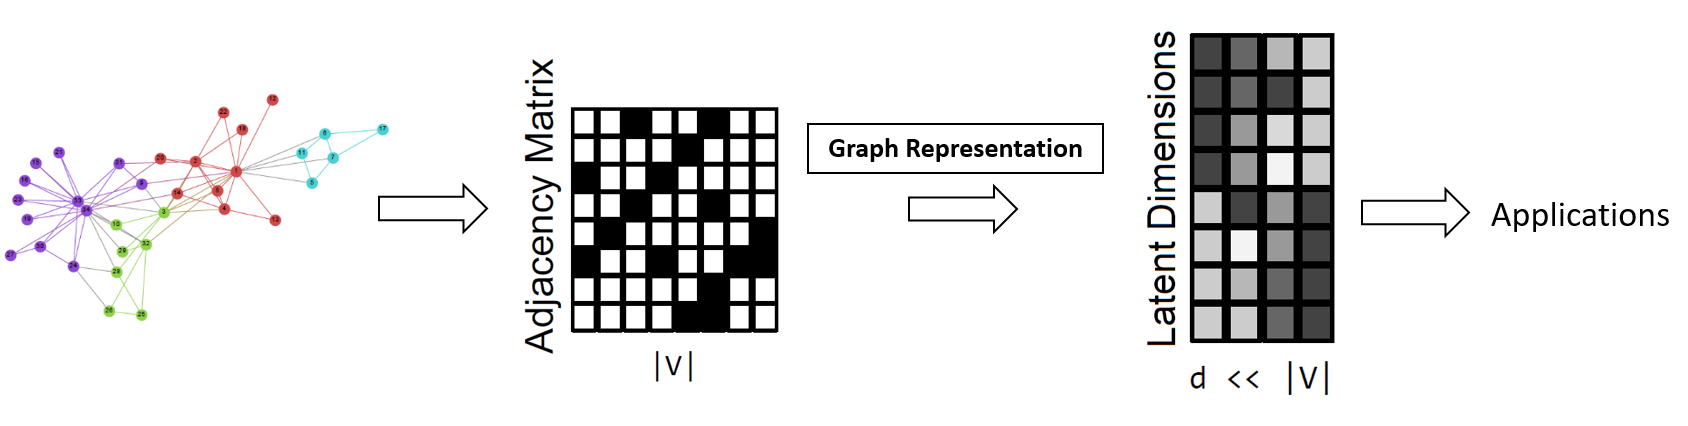
\includegraphics[width=5.5in]{figures/network_embedding}
	\caption{图表征算法}
\end{figure}


网络的邻接矩阵随着图中节点规模的增大,会变得非常稀疏,也就显现出了低秩的性质。对于低秩矩阵的流形学习的思想类似于图表征的过程。流形学习(Manifold Learning)领域提出借鉴拓扑流形的降维方式,这些方法通过设计一些表示节点间关系的矩阵,通过特征值分解的方法来获得表征向量,比如最基础的用来表示节点之间关系的邻接矩阵$A$,拉普拉斯矩阵 $L$(Laplacian Matrix)。通过分析,适用特征值分解的方式,需要矩阵满足对称正定,对于设计不符合要求的矩阵则需要根据随机梯度下降(Stochastic Gradient Descent)去求解。
在2013年,Google的开源工具Word2Vec\cite{mikolov2013efficient}发布之后,借鉴词向量表征的思路,Node2Vec和DeepWalk算法以蒙特卡罗随机游走的方式进行网络路径采样,将采样得到的路径视为词向量表征中的语料库,然后采用类似Word2Vec方法进行学习。在2015年,Jian Tang\cite{tang2015line}在提出LINE算法的同时提出了接近度的概念,根据接近度的概念,可以将不同的图表征算法进行分类。下面主要介绍一下接近度的概念,然后基于接近度的阶数,按从低阶到高阶接近度依次介绍:局部线性嵌入LLE(Locally Linear Embedding),拉普拉斯映射LE(Laplacian Eignemaps) , LINE(Large-scale Information Network Embedding)算法, DeepWalk算法,Node2Vec算法。
\subsection{接近度}
\begin{itemize}
	\item \textbf{一阶接近度}
	\item \textbf{二阶接近度}
\end{itemize}




%%%%%%%%%%%%%%%%%%%%%%%%%%%%%%%%%%%%%%%
%---------------------------------------     本章小结     ----------------------------------------%
%%%%%%%%%%%%%%%%%%%%%%%%%%%%%%%%%%%%%%%
\section{本章小结}
本章对本文相关的研究工作进行调研,分别从函数与程序库推荐、相似移动应用检测两个方面对现有的相关文献和工作进行分析和讨论。由于本文研究的问题——为开发者推荐合适的第三方库——鲜有相应工作,因此本章对与本文相近的工作进行调研分析。

函数和程序库推荐与本文研究问题相近,其主要目的是在项目工程开发过程,为开发者推荐合适、正确的函数、参数等,以避免错误使用和程序漏洞。相关的程序库推荐主要面向的是传统项目工程(如Java、C\#等),且通过分析项目中已使用的程序库情况,为开发者推荐其他相关的程序库。而本文研究的对象是移动应用,且关注分别在需求分析和后期维护两个阶段对开发者需求进行分析,从而为开发者推荐最合适最优的第三方库。本文研究的场景更广,且主要面向移动应用开发者。

相似移动应用检测是本文研究算法中的重要组成部分,因此本章调研了相关工作,并与本文提出的相似性计算方法进行比较和讨论。在相似移动应用检测工作中,主要分为两类方法,分别是动态检测和静态检测。由于动态检测方法需要在运行环境下对移动应用进行检测,因此需要消耗大量的计算资源,难以在大规模的移动应用数据库上进行扩展和应用。静态检测方法通常从移动应用元数据和程序代码两个角度进行分析检测。移动应用元数据包含多种数据类型,能够表征移动应用的功能特征,特别是描述文本,其通常阐述了与移动应用功能相关的文字信息。但此类方法忽略了移动应用代码层信息,特征涵盖不全,因此在相似性计算中可能有偏差。程度代码则从底层、更细粒度的角度体现了移动应用的功能信息,通过分析程序中各函数间的依赖关系,能够提取移动应用在代码层面的特征。但在程序依赖图构建过程中,需要消耗大量计算资源,无法实现快速高效识别。

现有的方法,多仅从元数据或程序代码角度对移动应用进行相似性分析,鲜有同时从本文和视图两个角度对移动应用进行特征提取,因此本文将在第四章中给出本文提出的基于文本和视图的移动应用相似性计算,从而为开发者推荐合适优质的第三方库。




	